%\documentclass{acm_proc_article-sp}
\documentclass{sig-alternate}
\newtheorem{definition}{Definition}
\usepackage{paralist}
\usepackage{url}
\usepackage{graphicx}
\usepackage{amsmath,amssymb}
\usepackage{listings}
\usepackage[dvipsnames]{xcolor}
\usepackage{tikz}
\usetikzlibrary{trees}


\newcommand\ednote[1]{\typeout{There is still an editor's note!!!}%
  \footnote{EDNOTE: #1}}
\newcommand\edbf[1]{\typeout{There is still an editor's note!!!}%
  \textbf{EDNOTE: #1}}

\def\collapse#1{\textcolor{blue}{\ensuremath{\mathord{\blacktriangleleft}
\mathord{#1}
\mathord{\blacktriangleright}}}}

% \DeclareUnicodeCharacter{B1}{\pm}
%% LANGUAGE      Markup definitions
\def\lstxml{
  \lstset{language=XML,
    basicstyle=\scriptsize,
    keywordstyle=\bfseries\ttfamily,
    identifierstyle=\ttfamily, 
    % commentstyle=\color{Brown},
    stringstyle=\ttfamily,
    showstringspaces=false,
    columns=[l]flexible, %% , basewidth={0.5em,0.4em}
    escapeinside={(@*}{*@)},
    deletekeywords={type,id}, % does not work!
    otherkeywords={encoding,
      mrow,math,mfrac,mi,msqrt,mo,mn,span,nobr,img,msup,maction,mtext}
  }
}
\def\lsthtml{
\lstset{language=html,
    basicstyle=\scriptsize,
    keywordstyle=\bfseries\ttfamily,
    showstringspaces=false,
    % otherkeywords={mfenced, open, close, separators, mrow, mi, mo, mn, math, 
    %   msup, role, parent, children, added}
}
}

\def\latex{\LaTeX}


\begin{document}
\CopyrightYear{2016} 
\setcopyright{acmcopyright}
\conferenceinfo{W4A'16,}{April 11-13, 2016, Montreal, Canada}
\isbn{978-1-4503-4138-7/16/04}\acmPrice{\$15.00}
\doi{http://dx.doi.org/10.1145/2899475.2899494}


\title{Adaptable Accessibility Features for Mathematics on the Web}
  

\numberofauthors{3}
\author{
  \alignauthor {Davide Cervone}\\
  \affaddr{MathJax Consortium}\\
  \affaddr{Union College, NY}\\
  \email{\normalsize dpvc@union.edu}
  %
  \alignauthor{Volker Sorge}\\
  \affaddr{MathJax Consortium}\\
  \affaddr{University of Birmingham, UK}\\
  \email{\normalsize V.Sorge@cs.bham.ac.uk}\\
  %% Thanks does not seem to work.
}

\maketitle

\begin{abstract}
  Assistive technology support for mathematical expressions has always been a
  challenging problem, which is not only compounded by the fact that there exist
  multiple markup languages in which to represent formulas as well as multiple ways to
  describe the same, visually equivalent formula even in the same markup
  language, but also that users have different needs, different levels of
  expertise and work with material from different subject areas.

  In MathJax, a Javascript library for TeX-like typesetting of Mathematics on the
  web,

  The new version will allow for a multitude 

  Since its beginnings one of its goals is to provide accessibility support for
  blind and visual impaired people; either by supporting third party assistive
  technology or, more recently, via it's own integrated accessibility extension.
In MathJax's new version 3 the accessibility extension is not only again an
important aspect but has been considerably improved in terms of the information
it can provide on formulas.

Another emphasis is to provide better accessibility to advanced mathematical
material exploiting information gained from the original LaTeX code, to provide
more appropriate speech for different areas of Mathematics but also for subjects
like Physics, Chemistry and Logic.  Our aim is to ease the study of mathematics
for more people with visual impairments as well as to encourage subject
specialists to contribute via better authored content, semantically meaningful
LaTeX packages, and expert knowledge for speech generation.
\end{abstract}

\keywords{STEM Accessibility, Mathematics, MathJax}


\enlargethispage{10pt}
\section{Introduction}

With more and more mathematical teaching material being made available online,
its accessible representation is a major concern. And while formulas on the web
can be represented in MathML~\cite{MathML3}, no major browser completely
implements this standard. Consequently the MathJax library that provides a
solution to render Mathematics in any browser, has become a quasi-standard for
displaying Mathematics on the web.  MathJax is a Javascript library for TeX-like
typesetting of Mathematics on the web. Since its beginnings one of its goals is
to provide accessibility support for blind and visual impaired people; either by
supporting third party assistive technology or, more recently, via it's own
integrated accessibility extension.

In MathJax's new version 3 the accessibility extension is not only again an
important aspect but has been considerably improved in a number of important
ways.


terms of the information
it can provide on formulas. With support from the Simons Foundation we developed
improved semantic recognition of source material as well as means to exploit
context information in documents. One particular emphasis is to provide better
accessibility to advanced mathematical material exploiting information gained
from the original LaTeX code, to provide more appropriate speech for different
areas of Mathematics but also for subjects like Physics, Chemistry and Logic.
Our aim is to ease the study of mathematics for more people with visual
impairments as well as to encourage subject specialists to contribute via better
authored content, semantically meaningful LaTeX packages, and expert knowledge
for speech generation.


  In MathJax, a Javascript library for TeX-like typesetting of Mathematics on the
  web,

  Since its beginnings one of its goals is to provide accessibility support for
  blind and visual impaired people; either by supporting third party assistive
  technology or, more recently, via it's own integrated accessibility extension.
In MathJax's new version 3 the accessibility extension is not only again an
important aspect but has been considerably improved in terms of the information
it can provide on formulas.

Another emphasis is to provide better accessibility to advanced mathematical
material exploiting information gained from the original LaTeX code, to provide
more appropriate speech for different areas of Mathematics but also for subjects
like Physics, Chemistry and Logic.  Our aim is to ease the study of mathematics
for more people with visual impairments as well as to encourage subject
specialists to contribute via better authored content, semantically meaningful
LaTeX packages, and expert knowledge for speech generation.


Personalisation aspects:


\begin{itemize}
\item Automatic voicing of formulas
\item Interactive navigation with synchronised highlighting
\item Different collections of speech rules like MathSpeak and ClearSpeak
\item Nemeth Braille output
\item Subject specific voicing for advanced mathematics
\item Different magnification and zoom engines
\item Variety of highlighting styles
\end{itemize}

All this depends on a rich semantic representation of mathematical formulas.


Also MathJax can render the three most common markup language for Mathematics
--- {\LaTeX}, ASCIIMath, and MathML --- neither has sufficient semantic
information to easily allow for the generation of meaningful speech,
explanations or subject specific highlighting.




The current state of mathematics support on the web is in a sad state of
affairs.  Although Mathematical formulas on the web can be represented in their
own specialized markup language, MathML~\cite{MathML3} as part of the HTML5
standard~\cite{HTML5}, only very few major browsers implement MathML rendering
natively, leading to sketchy support for displaying formulas included in pure
MathML on web pages.  Those browsers that do provide MathML support generally
only offer it partially, or lack its full integration into other technologies of
the Open Web Platform (OWP). For example, Firefox does not implement the
\texttt{GlobalEventHandler} API and has inconsistent support for Cascading Style
Sheets (CSS) on MathML elements. While Safari has a more modern integration into
the standard interfaces for the DOM (the tree structure representing the HTML
document), it does not implement all MathML elements, such as \texttt{maction},
and it collapses line-broken content onto the same line.  While neither Mozilla
nor Apple are actively developing the MathML support in their browsers, other
browser vendors like Google~(Chrome) and Microsoft~(IE/Edge), or 55\%-75\% of
the browser market, list MathML support as simply not planned.

It would be unfair, however, to blame the current lack of MathML support on the
browser vendors alone. Equal blame must fall on the failure of standardization
efforts at the W3C to pro-actively advance MathML in the face of developments in
other OWP standards, and to adapt it to the modern realities of browser
rendering and web programming. MathML is underspecified in terms of describing
layout rules, but more importantly, it lacks corresponding modules in CSS and
ARIA (assistive technology standards) to clarify implementation details for math
layout and semantics in browser engines.  In addition, some layout features are
incompatible with their corresponding CSS.  For example \texttt{mtable}
layout has simultaneously more (e.g., labeled rows), less (e.g., border
options), and incompatible (relative spacing) features compared to regular HTML
\texttt{table}s.  Similarly, \texttt{mpadded} is incompatible with CSS
\texttt{padding}.  Yet we also see features of math layout being subsumed by
modern CSS technology (e.g., flexbox) and re-invented in upcoming standards
(e.g., in-table alignments).  Thus we can expect more incompatibilities with
existing specifications in the future.
% https://drafts.csswg.org/css-text-4/#character-alignment

While MathML is a markup language for both the syntactic composition of
expressions via Presentation MathML and highly specialized semantic
representation via Content MathML, that will certainly continue to be used in
publishing workflows, its future as a web standard is doubtful.  As a
consequence, authors of mathematical web content and platforms supporting
mathematical authoring rely on JavaScript libraries such as
MathJax~\cite{MathJax2.5} to ensure flawless rendering of formulas across all
platforms and browsers.

Given the sad state of visual rendering of math on the web, it is of little
surprise that the web accessibility of math is even worse.  Before 2012, math
accessibility on the web was synonymous with
MathPlayer~\cite{soiffer2005mathplayer} on Internet Explorer. With IE11
deprecating plugins like MathPlayer, and with ChromeVox~\cite{Sorge14} and
VoiceOver~\cite{voiceover} adding some MathML support, the landscape has grown more
complex. Unfortunately, the core problem for web-based math accessibility has
not changed: browsers offer very limited MathML support. Consequently, the
majority of assistive technology solutions on the market today rely to some
degree on the ability of MathJax to turn Mathematics on the web into a uniform
MathML representation regardless of whether its source is in {\LaTeX}, ASCIIMath,
or MathML notation.

It is therefore a natural step to turn MathJax into a \emph{Universal Rendering
  Solution}. That is, making it an inclusive software solution in the
\emph{Universal Design} sense, rendering mathematics in a way that makes it
accessible to a wide spectrum of readers, regardless of their disabilities,
while retaining the same quality and user experience, regardless of the
platform, browser, or assistive technology solution employed by a user.  The
basis forms a uniform semantic enrichment of MathML expression (presented in
\S\ref{sec:semantic-enrichment}) that allows us to implement a number of
accessibility features (\S\ref{sec:at-solution}). However, our requirement to be
a platform independent solution, leads to a number of technical challenges and
suggestions for future developments and standards to enhance STEM accessibility
on the web, which we discuss in \S\ref{sec:challenges}.

\section{Semantic Enrichment}
\label{sec:semantic-enrichment}

\begin{figure}[t]
  \quad
  \begin{minipage}{.35\columnwidth}
\begin{lstlisting}[language=TeX,basicstyle=\scriptsize]
  ax^2 + b + c = 0
\end{lstlisting}
\begin{lstlisting}[language=XML,basicstyle=\scriptsize]
  <math>
    <mi>a</mi>
    <msup>
      <mi>x</mi>
      <mn>2</mn>
    </msup>
    <mo>+</mo>
    <mi>b</mi>
    <mi>x</mi>
    <mo>+</mo>
    <mi>c</mi>
    <mo>=</mo>
    <mn>0</mn>
  </math>
      \end{lstlisting}
    \end{minipage}
  \qquad
\begin{minipage}{.6\columnwidth}
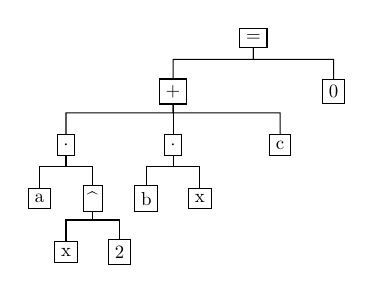
\begin{tikzpicture}[scale=.68, transform shape,
  level 1/.style={level distance=.8cm}
  ]
  \node[draw] {=}
  [grow via three points={one child at (0,-1.25) and two children at
(-1.5,-1) and (1.5,-1)}, edge from parent fork down]
  child {node[draw] {+}[grow via three points={one child at (0,-1) and
two children at (-1,-1) and (1,-1)}, edge from parent fork down]
  child {node[draw] {$\cdot$}[grow via three points={one child at
      (0,-1) and two children at (-.5,-1) and (.5,-1)}, edge from parent fork 
down]
    child {node[draw]{a}}
  child {node[draw] {$\,\widehat{}\,$}[grow via three points={one
      child at (0,-1) and two children at (-.5,-1) and (.5,-1)}, edge from parent 
fork
    down]
    child {node[draw]{x}}
    child {node[draw]{2}}}
        }
  child {node[draw] {$\cdot$}[grow via three points={one child at
      (0,-1) and two children at (-.5,-1) and (.5,-1)}, edge from parent fork 
down]
    child {node[draw]{b}}
    child {node[draw]{x}}
        }
  child {node[draw]{c}}
        }
  child {node[draw] {0}}
  ;
\end{tikzpicture}
  \end{minipage}
  \caption{Quadratic equation $ax^2 + bx + c = 0$ in presentation
    MathML and as semantic term tree.}
  \vspace*{-.3cm}
  \label{fig:semantic-tree}
\end{figure}

One of the main challenges for turning MathJax into a universal renderer is that it
was originally designed exclusively for displaying formulas, offering
a number of different rendering solutions, such as HTML with CSS or SVG. Thus,
although MathJax uses MathML as its internal format, expressions in the DOM are
collections of \texttt{div} and \texttt{span} elements or SVG graphics elements, which often
retain very little of the structure of the MathML tree they represent.

A second problem stems from the semantic weakness of Presentation MathML,
which contains relatively little mathematical information. In particular, MathML
expressions are often geared towards display, and so omit or obscure much of
the actual mathematical structure.

We have overcome these problems by imposing a ``light'' semantic interpretation
on math expression and generating a tree representation that can be embedded
into rendered MathJax expressions to ensure a similar user experience across
browsers. The idea of the semantic interpretation is an extension of the
heuristics implemented in the screen reader ChromeVox~\cite{Sorge14}, which
effectively rewrites a flat MathML expression into a term tree structure by first
interpreting the basic nature of symbols and propagating this through the
expression to determines the scope of operators, relations, etc.
Figure~\ref{fig:semantic-tree} presents this transformation for the example of
the quadratic equation $ax^2 + bx + c = 0$, which is rewritten from its
Presentation MathML form in the middle into its semantic interpretation on the
right.

The resulting semantic tree can be understood as an orthogonal view of the mathematical
expression, and we make concrete use of it by embedding it as \texttt{data}
attributes within MathJax's internal MathML representation. This then allows
MathJax's various renderers to push these data attributes into the actual
rendering elements used in the DOM, thus retaining the semantic tree structure
and making it available within the page.
Data attributes provide a fast and standardized means of retrieving information
from the DOM that is fully consistent with HTML5 practices.


\section{Assistive Technology Support}
\label{sec:at-solution}


The assistive technology extension that we have built for MathJax is mainly
aimed at supporting users with reading disorders, such as dyslexia, and visual
impairments. However, some aspects if it could also be used as a general aid for readers
unfamiliar with the content or for learners at different levels. We summarize the
main features in this section.

\subsection{Highlighting}

Mathematical expressions generally are large collections of mostly unconnected
symbols in a two-dimensional layout that can be particularly daunting for
readers with dyslexia.  Reading comprehension can be supported, 
however, by a
choice of high-contrast colors~\cite{rello2012optimal} and selective
highlighting~\cite{jones2008strategies}. We realize this in MathJax by offering
changes of fore- and background colors, and selective highlighting of
sub-expressions of a complex formula. We again exploit the semantic
structure of the formula to provide a more meaningful highlighting, as the
following example demonstrates (it is the first line of the example given in
Fig.~\ref{fig:collapse}) by contrasting the syntactic highlighting above against
the semantic highlighting below; every other element is highlighted.
\def\cb#1{\colorbox{yellow}{\ensuremath{\!\!\displaystyle#1\!\!}}}
{\skip0=\baselineskip \small\baselineskip=\skip0
\[\cb{I_\nu}
  (
  \cb{\nu^{-1}}
  ,
  \cb{1}
  )
  \mathrel{\cb{=}}
  \frac{\pi^2}{4}
  \mathop{\cb{\ln}}
  \left(
    \cb{\tfrac{(1+\nu)^{1+\nu}}{\nu^\nu}}
  \right)
  \mathbin{\cb{-}}
  \frac{7\zeta(3)}{8}
  \cb{\nu}
  +
  \cb{2}
  \int^\frac{1-\nu}{1+\nu}_1
  \cb{\frac{\chi_3(v)}{(1+v)^2}}
  {\rm d}
  \cb{v}
\]
\[\cb{I_\nu(\nu^{-1},1)}
  =\cb{\frac{\pi^2}{4}\ln\left(\tfrac{(1+\nu)^{1+\nu}}{\nu^\nu}
\right)}-\cb{\frac{7\zeta(3)}{8}\nu}+
\cb{2\int^\frac{1-\nu}{1+\nu}_1\frac{\chi_3(v)}{(1+v)^2}{\rm d}v}
\]
}

\enlargethispage{10pt}
In practice, sub-expressions are highlighted when hovering over them with the
mouse pointer, or by switching highlighting on permanently. This can be
recursively refined for sub-expressions, e.g., hovering on the denominator or
numerator of a fraction only. For permanent highlighting, the opaqueness of the
background gradually increases in nested sub-expressions. Nevertheless, in large
expressions, highlighting is of limited utility in getting an overview of the structure
of a formula; to aid this further, we introduce a technique for
structural abstraction in the next section.

\subsection{Structural Abstraction}
\label{sec:abstraction}

\begin{figure*}[t]
  \begin{minipage}{1.05\columnwidth}
    \centering
    % 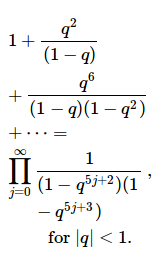
\includegraphics[width=\textwidth]{linebreaking}
  \end{minipage}
  \begin{minipage}{.1\textwidth}
    \begin{align*}
      \collapse{\mathrm{f}()} & = \collapse{+} \\
                              & = \collapse{+} \\ 
                              & = \collapse{+} \\ 
                              & = \collapse{+} + \collapse{\cdot} + \collapse{\cdot} \\
                              & \collapse{...} 
    \end{align*}
  \end{minipage}
  \begin{minipage}{.25\textwidth}
    \centering
    % 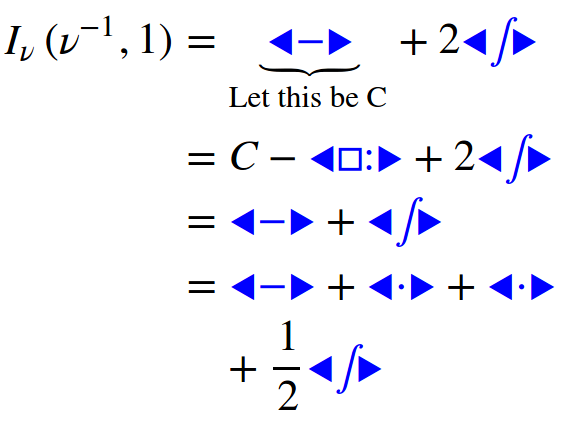
\includegraphics[width=\textwidth]{expand1}
  \end{minipage}\qquad\quad
  \vspace*{-.2cm}
  \caption{Two abstractions of the complex equation system on the left.}
  \vspace*{-.3cm}
  \label{fig:collapse}
\end{figure*}


The idea of structural abstraction is to assist readers by simplifying
the structure of the formula initially and letting them individually explore the
equation by manually expanding selected sub-expressions.  We have implemented
this via a user interface based on MathML's \texttt{maction} element
(cf.~\cite[3.7.1]{MathML3}). It allows users to explore the content using click,
keyboard, and touch events. The \texttt{maction} elements are nested so that only
the next level of the collapse is revealed.  The element indicating collapsed
content is a simple Unicode construction, \collapse{X}, with X indicating the
top-level structure that was collapsed. For example we use \collapse{+} to
indicate a sum, \collapse{\mathrm{\int}} an integral, etc.

Fig.~\ref{fig:collapse} demonstrates three different states of collapse of our
example equation.  To determine which parts are collapsed, our algorithm
somewhat surprisingly does not calculate sub-expression width, since these are
not available before rendering. Instead, it estimates the complexity of an
expression by recursively evaluating the enriched MathML tree. For example,
token elements are assigned a complexity value according to their string content
while more complex elements such as roots or fractions are assigned the sum of
their children's complexity measures modified by a value corresponding to their
own visual complexity. Cut-off values for each semantic type are then used to
decide which expressions are collapsed. The parameters (character weight,
operator modifier, cut-off) are configurable by the author.

\subsection{Aural Rendering}

To support screen-reader users, but make them independent of their particular
screen-reader's Math capabilities, MathJax now exploits direct access to the
speech-rule engine~\cite{Sorge14} that generates the semantic-tree
transformation in the first place and provides aural rendering of mathematical
expressions that can be directly exposed to a screen reader. Speech string
computation is based on the embedded semantic tree and uses the MathSpeak rule
set~\cite{MathSpeak}. Speech strings for a formula are either
pre-computed and embedded as another data attribute, or generated on the fly. 

To expose the speech strings to a screen reader, MathJax introduces a dedicated assertive ARIA
live region into the DOM and updates it with the desired speech output.
Speech strings can be computed not only for an entire formula, but also
for all its sub-expressions, which is helpful for interactive exploration.  We 
describe this next.




\subsection{Interactive Exploration}

Since mathematical formulas are generally of a complex nature, and already a
small formula can make for a complex utterance, just listening to an expression
once generally is not enough for comprehension. It is particularly
important, therefore, to provide the reader with a means of engaging with formulas
interactively. MathJax offers an interface for interactive exploration
of mathematical expressions that allows a reader to step through sub-expressions
either along the syntactic structure or the semantic tree.

Technically, this is realized by giving each math expression an ARIA role of
\texttt{application}, and upon entering an expression, the user can walk it using the
cursor keys. Exploration is supported by both highlighting and voicing
sub-expressions under consideration, where the former is achieved by updating
CSS properties of elements and the latter by updating the ARIA live region
introduced in the DOM.  Again, since the walking is effectively based on the
embedded semantic structure, the user experience of exploring a structure is the
same regardless of the specific renderer used.

\subsection{Braille Support}

currently we have only Nemeth Braille implemented but we plan to add more styles
in the future.


\subsection{Magnification}

While changing contrasts can already help low-vision users, many rely on screen
magnification to read content.  MathJax supports magnification in multiple ways:
standard browser zoom is supported by re-rendering mathematics at the new size.
MathJax also provides global scaling settings to enlarge all math
elements at once.  Individual math expressions can be further magnified using a
``lens'' that ordinarily offers a zoom window on top of an expression, with
scrolling to pan across the entire zoomed expression. Exploiting the semantic markup,
this lens can be restricted to particular sub-expressions only as for instance
in the example below.

\qquad\qquad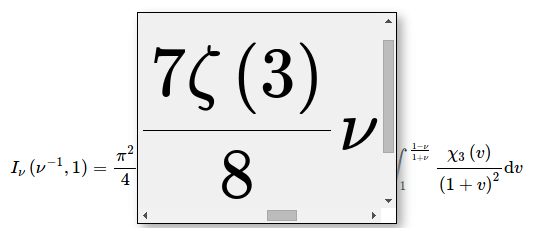
\includegraphics[height=2.2cm]{zoom}

On small devices, zooming usually is not beneficial, as it leads to overflow and
two-dimensional scrolling.  For magnification, it is possible to avoid excessive
scrolling or panning by re-flowing with line-breaks; but applying line-breaking
programmatically to long or complex equations often destroys their readability
due to cluttered results. We exploit the semantically enriched markup to perform
line-breaks at mathematically appropriate positions only. While this can
occasionally lead to less optimal usage of screen real-estate, it does
significantly help readability of formulas and also yields good results on small
form factors.

\subsection{Formula Colouring}

Tree-colouring
    Example: \[\color{blue}{a}\color{OliveGreen}{x^2}\color{red}{+}\color{blue}{b}
    \color{OliveGreen}{x}\color{red}{+}\color{blue}{c}\color{black}{=}\color{magenta}{0}\]


\section{Adaptation and Personalisation}
\label{sec:challenges}


which allow the user to adapt the 

but also a pick and mix of multiple assistive features.

speech adaptation

Domain adaptation by choice of heuristics

Automatic 

\section{Conclusions}
\label{sec:conc}

We have presented the new accessibility features of MathJax that aim to
transform MathJax into a universal rendering solution supporting all readers,
regardless of their disabilities. The features are based on a new semantic
enrichment procedure for Presentation MathML, which not only ensures a uniform
user experience across platforms and render solutions, but also shows promise
for more advanced AT techniques in the future. The presented AT extensions are
not yet available in core MathJax, but will be released as a MathJax extension
usable with current MathJax versions and possibly become part of MathJax's core
in version 3.0.


%   We therefore believe that our work can be
% significantly expanded, by
% \begin{inparaenum}[(1)]
% \item enhancing the precision of the semantic analysis, 
% \item adding subject specific rules, or 
% \item harvesting semantics from surrounding context.
% \end{inparaenum}

Although we have not yet had the opportunity to do extensive user testing, since
our code is developed publicly on our GitHub repository, we have already had
some user feedback, in particular from specialists, where initial reactions have
been positive. Additional end user testing was enligthening. Users struggled 
with lack of live-regions support in their AT and the complexity of the 
application. Feedback indicates that options for additional speech styles and 
semantics will be beneficial. 
We spent a significant effort on
technical testing in order to make the solution compatible with the most common
assistive technology solutions. 
We strongly believe that these experiences and
the observed shortcomings, should serve as a use case for the future development
of standards, tools and general accessibility solutions for STEM content the
web. 







\begin{thebibliography}{1}\small

\bibitem{voiceover}
Voiceover.
\newblock \url{apple.com/accessibility/osx/voiceover}.

\bibitem{HTML5}
% R.~Berjon, S.~Faulkner, T.~Leithead, E.~Doyle Navara, E.~O'Connor, S.~Pfeiffer, I.~Hickson.
\newblock {HTML} v5.0.
\newblock W3C recom., 2013.
\newblock \url{www.w3.org/TR/html5}.

\bibitem{MathML3}
D.~Carlisle, P.~Ion, R.~Miner.
\newblock {MathML} v3.0.
\newblock W3C recom., 2010.
\newblock \url{www.w3.org/TR/MathML3}.

\bibitem{MathJax2.5}
\newblock {MathJax} v2.5, 2014.
\newblock \url{www.mathjax.org}.

\bibitem{jones2008strategies}
R.~Jones.
\newblock Strategies for reading comprehension: Selective underlining, 2008.

\bibitem{MathSpeak}
A.~Nemeth.
\newblock Mathspeak.
\newblock \url{www.gh-mathspeak.com}, 2005.

\bibitem{rello2012optimal}
L~Rello and R~Baeza-Yates.
\newblock Optimal colors to improve readability for people with dyslexia.
\newblock In {\em Text Customization for Readability Symposium}, 2012.

\bibitem{soiffer2005mathplayer}
N.~Soiffer.
\newblock Mathplayer: web-based math accessibility.
\newblock In {\em 7th Computers and Accessibility Conf.}, 2005. ACM.

\bibitem{Sorge14}
V.~Sorge, C.~Chen, T.V.~Raman, D.~Tseng.
\newblock Towards making mathematics a first class citizen in general screen
  readers.
\newblock In {\em 11th Web for All Conf.}, 2014. ACM.

\bibitem{Sorge15}
V.~Sorge, M.~Lee, S.~Wilkinson.
\newblock End-to-end solution for accessible chemical diagrams.
\newblock In {\em 12th Web for All Conf.}, 2015. ACM.

\end{thebibliography}

% \pagebreak
% \begin{itemize}
% \item first comment: "My main concern with the paper is the lack of evaluation of the proposed features. Although extensive testing is listed as one of the challenges, due to the lack of adequate tools, a few evaluations based on user observation would already provide invaluable feedback to help improve each feature and MathJax as a whole."
% \item Peter: user feedback was sought but is still being overshadowed by the limitations of the platform (see below)
% \item Peter: user feedback negative in this sense: too hard to understand when to drop out of modes, how to interact, how to know AT well enough to get the benefits
% 
% \itme Limited end user testing was more. Users struggled with lack of 
% live-regions support and the complexity of the application. Inexperience with 
% voicing and exploration of mathematical content made it difficult for them to 
% assess the quality of the results.
% 
% \item second comment "it would have been even stronger had it been able to more generally extrapolate from this experience to the sorts of challenges that would be encountered in adding analogous extensions to other interfaces."
% \item Volker: write about generalization for similar STEM apps -- quote V's chemistry paper
% \item Volker: write what would be nice  / good to know for similar endeavors
% \item Peter: unclear implementation status of aria live regions (sometimes not announced, AT not leaving browse mode), AT feature "jump to last heard application and put focus on it; resume after leaving app" (in browse mode ) b/c in browse mode you pass an application with a label and you can't access it o
% \item Volker: automated tests and CI simply not possible 
% \item Peter: therefore increased development and maintenance costs, slowdown in feeding research into practice
% 
% \item third commment: "In fact, the practical approach of the paper is obvious, but it could excite more partners and collaborators, of the issues be shown as investigations or even if they were presented in a more scientific and contextualized way (for example, provoking developers to think about the levels of solutions they could be involved) ."
% \item Volker: see it as application engineering
% \item Volker: building rich web apps (menus, games) but apps on enriching content
% \item Volker: e.g., VO explains "applcation: press controle+alt+option+... to enter" but doesn't work becaue you're in the wrong mode.
% \end{itemize}

\end{document}


%%% Local Variables:
%%% mode: latex
%%% TeX-master: t
%%% End:
